\documentclass[10pt,letterpaper]{article}
\usepackage[utf8]{inputenc}
\usepackage[margin=0.5in]{geometry}
\usepackage{amsmath,amssymb}
\usepackage{multicol}
\usepackage{chemfig}
\usepackage{chemformula}
\usepackage{tikz}
\usepackage{enumitem}
\usepackage{fancyhdr}
\usepackage{booktabs}

\pagestyle{fancy}
\fancyhf{}
\lhead{2026 U.S. National Chemistry Olympiad}
\rhead{National Exam Part I}
\cfoot{\thepage}

\setlist[enumerate]{leftmargin=*, label=\bfseries\arabic*., itemsep=12pt, parsep=4pt}
\setlist[itemize]{leftmargin=*}

% Compact styling optimized for column-bounded organic structures
\setchemfig{atom sep=1.3em, label sep=2pt, bond offset=1pt, double bond sep=1.5pt, bond thickness=0.7pt}

\begin{document}

\begin{center}
    \textsc{\large 2026 U.S. National Chemistry Olympiad}\\
    \Large\textbf{NATIONAL EXAM PART I}
\end{center}
\vspace{0.2cm}

\begin{multicols*}{2}

\begin{enumerate}

    \item \ch{10.00 g} of blue copper sulfate pentahydrate, \ch{CuSO4 . 5 H2O}, is heated strongly to drive off all the water of hydration. How much colorless anhydrous copper sulfate remains?
    \begin{enumerate}[label=(\textsubscript{\Alph*})]
        \item 1.67 g
        \item 3.61 g
        \item 6.39 g
        \item 8.99 g
    \end{enumerate}

    \item Ethane reacts with oxygen according to the balanced equation below:
    \[ \ch{2 C2H6(g) + 7 O2(g) -> 4 CO2(g) + 6 H2O(l)} \]
    A mixture of ethane and oxygen occupies \ch{22.4 L} at STP. The mixture is allowed to react as described above, and the gases then occupy \ch{11.2 L} at STP. How many moles of ethane were originally present?
    \begin{enumerate}[label=(\textsubscript{\Alph*})]
        \item 0.20 mol
        \item 0.30 mol
        \item 0.40 mol
        \item It cannot be determined from the information given.
    \end{enumerate}

    \item \ch{0.2700 g} of a white solid is titrated with \ch{32.70 mL} of \ch{0.1834 M} \ch{NaOH} solution to achieve a phenolphthalein endpoint. Which is the molecular formula of the compound?
    \begin{enumerate}[label=(\textsubscript{\Alph*})]
        \item \ch{CHO2}
        \item \ch{CH2O2}
        \item \ch{C2H2O4}
        \item \ch{C2H4O4}
    \end{enumerate}

    \item Aqueous sodium hydroxide solutions absorb carbon dioxide both because carbon dioxide has an appreciable solubility in water and because the hydroxide ions react very favorably with excess \ch{CO2} to form bicarbonate ions.
    
    A rigid vessel with \ch{10.00 L} of headspace contains \ch{1.00 L} of \ch{0.100 M} \ch{NaOH} and is maintained at $25^\circ\text{C}$. Carbon dioxide is introduced into the headspace at a pressure of \ch{1.33 atm}, which decreases to \ch{1.00 atm} after absorption into the aqueous \ch{NaOH} is complete. If the experiment is repeated with an initial \ch{CO2} pressure of \ch{1.50 atm}, \ch{1.00 L} of what concentration of \ch{NaOH} would be required to reduce the pressure of \ch{CO2} to \ch{1.00 atm}?
    \begin{enumerate}[label=(\textsubscript{\Alph*})]
        \item 0.112 M
        \item 0.152 M
        \item 0.169 M
        \item 0.204 M
    \end{enumerate}

    \item What is the concentration of chloride ion in a solution prepared by mixing \ch{0.100 L} of \ch{0.100 M} \ch{LiCl} with \ch{0.200 L} of \ch{0.200 M} \ch{BaCl2} and \ch{0.300 L} of \ch{0.300 M} \ch{CeCl3}?
    \begin{enumerate}[label=(\textsubscript{\Alph*})]
        \item 0.200 M
        \item 0.233 M
        \item 0.467 M
        \item 0.600 M
    \end{enumerate}

    \item A U-tube is divided into two compartments by a semipermeable membrane that allows only water to pass through. On the left side of the U-tube is added \ch{10 mL} of \ch{0.20 M} sucrose solution and on the right side is added \ch{10 mL} of \ch{0.15 M} sodium chloride solution. Which best represents the appearance of the U-tube after equilibrium is attained?
    
    \begin{center}
    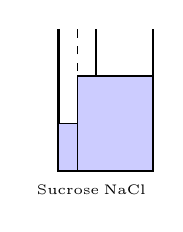
\begin{tikzpicture}[scale=0.6]
        \draw[thick] (0,3) -- (0,0) -- (2,0) -- (2,3);
        \draw[thick] (0.8,0) -- (0.8,3);
        \draw[dashed] (0.4,0) -- (0.4,3); 
        \node at (0.2,-0.4) {\tiny Sucrose};
        \node at (1.4,-0.4) {\tiny NaCl};
        \draw[fill=blue!20] (0,0) -- (0.4,0) -- (0.4,1) -- (0,1) -- cycle;
        \draw[fill=blue!20] (0.4,0) -- (2,0) -- (2,2) -- (0.4,2) -- cycle;
    \end{tikzpicture}
    \end{center}
    \begin{enumerate}[label=(\textsubscript{\Alph*})]
        \item Right side water level is higher than left side.
        \item Left side water level is higher than right side.
        \item Both sides remain perfectly equal in height.
        \item All liquid shifts completely to one side.
    \end{enumerate}

    \item A gas mixture extinguishes a glowing splint and does not cause limewater to turn cloudy when bubbled through it. Which most accurately describes the gas mixture?
    \begin{enumerate}[label=(\textsubscript{\Alph*})]
        \item It contains only carbon dioxide.
        \item It contains only oxygen.
        \item It contains both carbon dioxide and oxygen.
        \item It contains neither carbon dioxide nor oxygen.
    \end{enumerate}

    \item Which laboratory glassware is most useful for determining the melting point of a solid organic compound?
    \begin{enumerate}[label=(\textsubscript{\Alph*})]
        \item Thiele tube
        \item Liebig condenser
        \item Graduated cylinder
        \item Burette
    \end{enumerate}

    \item Which gas can be condensed to a blue liquid?
    \begin{enumerate}[label=(\textsubscript{\Alph*})]
        \item Carbon dioxide
        \item Hydrogen
        \item Nitrogen dioxide
        \item Ozone
    \end{enumerate}

    \item Which liquids are miscible in all proportions?
    \begin{enumerate}[label=(\textsubscript{\Alph*})]
        \item \ch{H2O} and \ch{CH2Cl2}
        \item \ch{H2O} and \ch{(CH3)2CO}
        \item \ch{C6H12} and \ch{Hg}
        \item \ch{C6H12} and \ch{CH3OH}
    \end{enumerate}

    \item Which is the best way to prepare \ch{0.5 L} of a \ch{1 M} solution of sulfuric acid?
    \begin{enumerate}[label=(\textsubscript{\Alph*})]
        \item \ch{0.5 mol} of concentrated sulfuric acid should be added to a \ch{500 mL} volumetric flask, followed by enough distilled water to fill the flask to the mark.
        \item \ch{0.5 mol} of concentrated sulfuric acid should be added slowly to about \ch{300 mL} of distilled water in a \ch{1 L} Erlenmeyer flask, then enough distilled water should be added to reach the \ch{500 mL} mark on the flask.
        \item \ch{11.2 L} of sulfur trioxide gas, measured at STP, should be bubbled through \ch{500 mL} of distilled water in a \ch{1 L} Erlenmeyer flask.
        \item To \ch{0.5 mol} of silver sulfate suspended in about \ch{300 mL} water in a \ch{500 mL} volumetric flask should be added \ch{1.0 mol} \ch{HCl}.
    \end{enumerate}

    \item A chemist determines the fraction of magnesium that burns in air to make \ch{Mg3N2} by adding the ash formed from a known mass of \ch{Mg} ribbon into water, distilling the mixture into a known excess of hydrochloric acid, and back-titrating the excess \ch{HCl} with \ch{NaOH} to a methyl orange endpoint. Which error will cause the calculated fraction of magnesium nitride to be too high?
    \begin{enumerate}[label=(\textsubscript{\Alph*})]
        \item The distillate is collected in a flask by itself and subsequently added to the \ch{HCl}.
        \item Phenolphthalein is used as an indicator in place of methyl orange.
        \item The potassium hydrogen phthalate used to standardize the \ch{NaOH} had absorbed some moisture from the air.
        \item When the \ch{HCl} solution was drawn into the volumetric pipet used to dispense it, a large bubble was present.
    \end{enumerate}

    \item \ch{H2O} has a higher normal boiling point than \ch{HF} ($100^\circ\text{C}$ vs. $20^\circ\text{C}$). Which is the best explanation for this difference?
    \begin{enumerate}[label=(\textsubscript{\Alph*})]
        \item \ch{H2O} has a larger dipole moment than \ch{HF}.
        \item \ch{H2O} is more polarizable than \ch{HF}.
        \item \ch{H2O} forms stronger hydrogen bonds than \ch{HF}.
        \item \ch{H2O} forms more hydrogen bonds per mole than \ch{HF}.
    \end{enumerate}

    \item A solution of camphor in benzene is cooled slowly to determine its freezing point. The thermal arrest curve displays significant supercooling followed by a stable plateau. What temperature should be reported as the true freezing point?
    \begin{enumerate}[label=(\textsubscript{\Alph*})]
        \item The absolute minimum temperature reached during supercooling.
        \item The temperature at the flat plateau after crystallization begins.
        \item The initial room temperature.
        \item The average of the start and end values.
    \end{enumerate}

    \item The vapor pressure of butane at $0^\circ\text{C}$ is \ch{1 atm}. A \ch{0.100 mol} sample of liquid butane at $0^\circ\text{C}$ is introduced into an evacuated, well-insulated \ch{2.25 L} container. Which statements correctly describe the system after it reaches equilibrium?
    \begin{itemize}
        \item[I.] The temperature is lower than $0^\circ\text{C}$.
        \item[II.] All of the butane is in the gas phase.
    \end{itemize}
    \begin{enumerate}[label=(\textsubscript{\Alph*})]
        \item I only
        \item II only
        \item Both I and II
        \item Neither I nor II
    \end{enumerate}

    \item The triple point of krypton is at \ch{0.73 bar} and \ch{116 K}. Which is true of a pure sample of \ch{Kr} at equilibrium at \ch{0.73 bar} and \ch{90 K}?
    \begin{enumerate}[label=(\textsubscript{\Alph*})]
        \item Only the gas phase is stable.
        \item Only the solid phase is stable.
        \item The solid and gas phases coexist.
        \item The solid and liquid phases coexist.
    \end{enumerate}

    \item Which statements about relative boiling points are correct?
    \begin{itemize}
        \item[I.] 2-Methylpropane has a higher normal boiling point than butane.
        \item[II.] 2-Methyl-1-propanol has a higher normal boiling point than 1-butanol.
    \end{itemize}
    \begin{enumerate}[label=(\textsubscript{\Alph*})]
        \item I only
        \item II only
        \item Both I and II
        \item Neither I nor II
    \end{enumerate}

    \item Gold crystallizes in a face-centered cubic lattice with a density of \ch{19.31 g cm^{-3}}. What is the radius of a gold atom?
    \begin{enumerate}[label=(\textsubscript{\Alph*})]
        \item 144.1 pm
        \item 176.5 pm
        \item 203.8 pm
        \item 288.2 pm
    \end{enumerate}

    \item Substance $R(g)$ reacts to form $P(g)$, which then may isomerize to either $P_1(g)$ or $P_2(g)$ as shown below:
    \[ R(g) \xrightarrow{\Delta G^\circ = -150\text{ J/mol}} P(g) \genfrac{}{}{0pt}{}{\nearrow \Delta G^\circ = +50\text{ J/mol } P_1(g)}{\searrow \Delta G^\circ = -50\text{ J/mol } P_2(g)} \]
    In an experiment, \ch{10.0 g} of $R(g)$ is placed in a sealed vessel. Which are true at equilibrium?
    \begin{itemize}
        \item[I.] The mass of $R(g)$ is 0.0 g.
        \item[II.] The mass of $P_1(g)$ is less than the mass of $P_2(g)$.
    \end{itemize}
    \begin{enumerate}[label=(\textsubscript{\Alph*})]
        \item I only
        \item II only
        \item Both I and II
        \item Neither I nor II
    \end{enumerate}

    \item \ch{60.0 mL} of \ch{0.60 M} \ch{HCOOH} and \ch{40.0 mL} of \ch{0.80 M} \ch{CH3NH2}, both initially at $22.0^\circ\text{C}$, are mixed in a well-insulated container. The final temperature is $27.9^\circ\text{C}$. What is $\Delta H^\circ_{\text{rxn}}$ for the reaction?
    \[ \ch{HCOOH(aq) + CH3NH2(aq) -> HCOO^{-}(aq) + CH3NH3^{+}(aq)} \]
    \begin{enumerate}[label=(\textsubscript{\Alph*})]
        \item $-31\text{ kJ mol}^{-1}$
        \item $-41\text{ kJ mol}^{-1}$
        \item $-69\text{ kJ mol}^{-1}$
        \item $-77\text{ kJ mol}^{-1}$
    \end{enumerate}

    \item What is $S^\circ$ for \ch{O2(g)} given the table below?
    \begin{center}
    \small
    \begin{tabular}{lccc}
        \toprule
        Species & $\Delta H^\circ_f$ & $S^\circ$ & $\Delta G^\circ_f$ \\
        \midrule
        \ch{H2O(l)} & -290 & 70. & -240 \\
        \ch{H2O2(l)} & -190 & 110. & -120 \\
        \bottomrule
    \end{tabular}
    \end{center}
    \begin{enumerate}[label=(\textsubscript{\Alph*})]
        \item $150\text{ J mol}^{-1}\text{ K}^{-1}$
        \item $210\text{ J mol}^{-1}\text{ K}^{-1}$
        \item $250\text{ J mol}^{-1}\text{ K}^{-1}$
        \item $290\text{ J mol}^{-1}\text{ K}^{-1}$
    \end{enumerate}

    \item Between \ch{293 K} and \ch{295 K}, \ch{Gd(s)} transitions from a ferromagnetic to a paramagnetic state, causing a significant anomaly in heat capacity. If heated at a constant rate, the temperature vs. heat graph will feature:
    \begin{enumerate}[label=(\textsubscript{\Alph*})]
        \item A transient drop in the slope due to the sudden jump in heat capacity.
        \item A perfectly flat horizontal line indicating a first-order phase transition phase.
        \item A sharp upward spike with infinite vertical derivative.
        \item No observable change.
    \end{enumerate}

    \item Which species has the greatest molar entropy $S^\circ$ at \ch{298 K}?
    \begin{enumerate}[label=(\textsubscript{\Alph*})]
        \item \ch{H2(g)}
        \item \ch{He(g)}
        \item \ch{Cl2(g)}
        \item \ch{Xe(g)}
    \end{enumerate}

    \item In an adiabatic process, no heat is exchanged with the surroundings. Which must be true in a reversible adiabatic process?
    \begin{itemize}
        \item[I.] $\Delta H = 0$
        \item[II.] $\Delta S = 0$
    \end{itemize}
    \begin{enumerate}[label=(\textsubscript{\Alph*})]
        \item I only
        \item II only
        \item Both I and II
        \item Neither I nor II
    \end{enumerate}

    \item The irreversible reaction of a compound A takes place with $\text{Rate} = k[A]^n$. The half-life of the reaction is independent of $[A]$. What is the value of $n$?
    \begin{enumerate}[label=(\textsubscript{\Alph*})]
        \item 0
        \item 1
        \item 2
        \item It cannot be determined from the information given.
    \end{enumerate}

    \item An acid-catalyzed reaction that is first-order in \ch{H+} has a rate of $5.0 \times 10^{-6}\text{ M s}^{-1}$ when carried out in a buffer with $\text{pH} = 5.0$. What is the rate when buffered at $\text{pH} = 5.5$?
    \begin{enumerate}[label=(\textsubscript{\Alph*})]
        \item $1.6 \times 10^{-6}\text{ M s}^{-1}$
        \item $4.5 \times 10^{-6}\text{ M s}^{-1}$
        \item $5.5 \times 10^{-6}\text{ M s}^{-1}$
        \item $1.6 \times 10^{-5}\text{ M s}^{-1}$
    \end{enumerate}

    \item The decomposition of hydrogen peroxide to form water and oxygen in the presence of an iodide catalyst is studied, and the rate law is found to be $\text{Rate} = k[\ch{H2O2}][\ch{I-}]$ with $k = 1.05\text{ M}^{-1}\text{ min}^{-1}$. A reaction is carried out with the initial concentrations of both iodide and hydrogen peroxide equal to \ch{0.300 M}. What is the concentration of hydrogen peroxide after \ch{5.00 min}?
    \begin{enumerate}[label=(\textsubscript{\Alph*})]
        \item 0.00157 M
        \item 0.0621 M
        \item 0.117 M
        \item 0.145 M
    \end{enumerate}

    \item The temperature dependence of the rate constant for the gas-phase reaction of acrolein with nitrate radical is measured, and the rate constant is found to be $k = (1.72 \times 10^{-13})\exp(-1190/T)$. What is the activation energy of the reaction?
    \begin{enumerate}[label=(\textsubscript{\Alph*})]
        \item $1.19\text{ total kJ mol}^{-1}$
        \item $9.89\text{ kJ mol}^{-1}$
        \item $36.4\text{ kJ mol}^{-1}$
        \item $143\text{ kJ mol}^{-1}$
    \end{enumerate}

    \item Which rate law is predicted by the following mechanism?
    \begin{align*}
        \ch{HCO2CH3(aq) + H+(aq)} &\rightleftharpoons \ch{HC(OH)(OCH3)+(aq)} \quad (\text{fast}) \\
        \ch{HC(OH)(OCH3)+(aq) + H2O(l)} &\xrightarrow{\text{slow}} \ch{HC(OH)(OH2)(OCH3)+(aq)}
    \end{align*}
    \begin{enumerate}[label=(\textsubscript{\Alph*})]
        \item $\text{Rate} = k[\ch{HCO2CH3}]$
        \item $\text{Rate} = k[\ch{HCO2CH3}][\ch{H+}]$
        \item $\text{Rate} = k[\ch{HCO2CH3}]/[\ch{H+}]$
        \item $\text{Rate} = k[\ch{H+}]$
    \end{enumerate}

    \item Which reaction coordinate diagram best corresponds to a mechanism containing one initial fast equilibrium followed by a single rate-determining slow step?
    \begin{enumerate}[label=(\textsubscript{\Alph*})]
        \item Small activation barrier peak followed by a very high second peak.
        \item Very high peak followed by a minor second peak.
        \item Single smooth parabolic peak.
        \item Three matching peaks in rapid succession.
    \end{enumerate}

    \item How much $\text{NaH}_2\text{PO}_4 \cdot 2\text{H}_2\text{O}$ must be added to \ch{400.0 mL} of \ch{0.200 M} \ch{H3PO4} to create a buffer solution with $\text{pH} = 2.30$? ($\text{p}K_{a1} = 2.12$)
    \begin{enumerate}[label=(\textsubscript{\Alph*})]
        \item 0.0144 mol
        \item 0.0529 mol
        \item 0.121 mol
        \item 0.303 mol
    \end{enumerate}

    \item Gaseous \ch{PCl5} decomposes to form \ch{PCl3} and \ch{Cl2}. At equilibrium, 20.0\% of the \ch{PCl5} has decomposed. Increasing the volume of the container by what factor will increase the percentage of decomposition to 50.0\% at equilibrium at this temperature?
    \begin{enumerate}[label=(\textsubscript{\Alph*})]
        \item 2.50
        \item 4.00
        \item 6.25
        \item 10.0
    \end{enumerate}

    \item Solid calcium carbonate is in equilibrium with calcium oxide and carbon dioxide, with $K_p = 0.12\text{ bar}$ at \ch{1200 K}.
    \[ \ch{CaCO3(s) <=> CaO(s) + CO2(g)} \]
    A \ch{1.00 g} sample of \ch{CaCO3} ($M = 100.09$) is placed in an evacuated piston which is allowed to equilibrate at \ch{1200 K}. How will the pressure in the piston depend on volume?
    \begin{enumerate}[label=(\textsubscript{\Alph*})]
        \item Remain constant at \ch{0.12 bar} until all \ch{CaCO3} decomposes, then decrease.
        \item Linear increase.
        \item Hyperbolic increase across all volumes.
        \item Zero pressure initially.
    \end{enumerate}

    \item A mixture of the diprotic acid \ch{HOC6H4COOH} and \ch{Na[HOC6H4COO]} is titrated with \ch{1.000 M} \ch{NaOH}. The titration curve exhibits two clear equivalence point jumps at \ch{2.0 mL} and \ch{8.0 mL}. Which statement is correct?
    \begin{enumerate}[label=(\textsubscript{\Alph*})]
        \item The ratio of the salt to the acid is 2:1.
        \item The total number of combined moles is 0.008.
        \item The $\text{p}K_{a1}$ is 5.3.
        \item The $\text{p}K_{a2}$ is 9.2.
    \end{enumerate}

    \item \ch{0.50 mol} of solid silver chloride ($K_{sp} = 1.8 \times 10^{-10}$) is added to \ch{1.0 L} of a \ch{0.100 M} solution of sodium bromide. What is the concentration of silver ion in solution at equilibrium? ($K_{sp}\text{ of AgBr} = 4.9 \times 10^{-13}$)
    \begin{enumerate}[label=(\textsubscript{\Alph*})]
        \item $4.9 \times 10^{-12}\text{ M}$
        \item $1.8 \times 10^{-9}\text{ M}$
        \item $7.0 \times 10^{-7}\text{ M}$
        \item $1.3 \times 10^{-5}\text{ M}$
    \end{enumerate}

    \item A solution is \ch{0.10 M} in both \ch{Cd^2+} and \ch{Tl+} and is kept saturated with \ch{H2S} gas ($[\ch{H2S}] = 0.1\text{ M}$). In what pH range will one metal ion precipitate quantitatively ($>99.9\%$) while the other remains completely in solution? ($K_{sp}\text{ CdS} = 1.0 \times 10^{-27}$, $K_{sp}\text{ Tl2S} = 6.0 \times 10^{-22}$)
    \begin{enumerate}[label=(\textsubscript{\Alph*})]
        \item Between 0.5 and 6.8
        \item Between 2.0 and 3.9
        \item Between 4.0 and 6.8
        \item There is no pH at which this is possible.
    \end{enumerate}

    \item \ch{NO} disproportionates into \ch{N2O} and \ch{NO2} in basic solution. When balanced using the smallest whole number coefficients, what is the coefficient of \ch{NO}?
    \begin{enumerate}[label=(\textsubscript{\Alph*})]
        \item 2
        \item 3
        \item 4
        \item 5
    \end{enumerate}

    \item Given the standard reduction potentials in basic solution:
    \begin{align*}
        \ch{MnO4^{-}(aq) + e^{-} -> MnO4^{2-}(aq)} &\quad E^\circ = 0.543\text{ V} \\
        \ch{MnO4^{-}(aq) + 2 H2O + 3e^{-} -> MnO2(s) + 4 OH^{-}} &\quad E^\circ = 0.595\text{ V}
    \end{align*}
    What is the standard reduction potential of the \ch{MnO4^{2-}(aq)/MnO2(s)} couple?
    \begin{enumerate}[label=(\textsubscript{\Alph*})]
        \item 0.052 V
        \item 0.569 V
        \item 0.621 V
        \item 0.647 V
    \end{enumerate}

    \item For the voltaic cell $\ch{Cr} | \ch{Cr^3+} \, (\ch{1.0 M}) || \ch{Ag+} \, (\ch{1.0 M}) | \ch{Ag}$, which change will cause the cell potential to decrease?
    \begin{enumerate}[label=(\textsubscript{\Alph*})]
        \item Decreasing the pH of the silver half-cell by adding concentrated nitric acid.
        \item Bubbling \ch{NH3(g)} through the silver half-cell.
        \item Adding water to the chromium half-cell.
        \item Increasing the size of the silver electrode.
    \end{enumerate}

    \item What is the molar solubility of lead sulfate at \ch{298 K}?
    \begin{align*}
        \ch{Pb^2+(aq) + 2e^{-} -> Pb(s)} &\quad E^\circ = -0.126\text{ V} \\
        \ch{PbSO4(s) + 2e^{-} -> Pb(s) + SO4^2-(aq)} &\quad E^\circ = -0.359\text{ V}
    \end{align*}
    \begin{enumerate}[label=(\textsubscript{\Alph*})]
        \item $1.31 \times 10^{-8}\text{ mol L}^{-1}$
        \item $8.46 \times 10^{-7}\text{ mol L}^{-1}$
        \item $5.46 \times 10^{-5}\text{ mol L}^{-1}$
        \item $1.14 \times 10^{-4}\text{ mol L}^{-1}$
    \end{enumerate}

    \item A solution containing a metal ion is electrolyzed, with \ch{1.50 g} of the metal being deposited at the cathode. Concurrently, \ch{0.265 L} of dry oxygen gas is collected at the anode (measured at STP). What is the metal?
    \begin{enumerate}[label=(\textsubscript{\Alph*})]
        \item Al
        \item Cu
        \item Sn
        \item U
    \end{enumerate}

    \item In a mercury Pourbaix diagram, which species occupies region X, located between $\ch{Hg^2+(aq)}$ at very low pH and $\ch{HgO(s)}$ at higher pH, under mild oxidizing potential conditions?
    \begin{enumerate}[label=(\textsubscript{\Alph*})]
        \item \ch{Hg2^2+(aq)}
        \item \ch{Hg2O(s)}
        \item \ch{Hg(OH)+(aq)}
        \item \ch{Hg(O)(OH)(s)}
    \end{enumerate}

    \item In which are the first ionization energies listed in increasing order?
    \begin{enumerate}[label=(\textsubscript{\Alph*})]
        \item $\ch{N < O < P < S}$
        \item $\ch{P < S < N < O}$
        \item $\ch{P < N < S < O}$
        \item $\ch{S < P < O < N}$
    \end{enumerate}

    \item The Balmer series lines correspond to transitions to $n_{\text{final}} = 2$. The longest wavelength is $\lambda = 656\text{ nm}$. Which of the following is NOT a member of the Balmer series?
    \begin{enumerate}[label=(\textsubscript{\Alph*})]
        \item 410 nm
        \item 434 nm
        \item 486 nm
        \item 545 nm
    \end{enumerate}

    \item The melting points of the group 6 elements increase down the group: $\ch{Cr} < \ch{Mo} < \ch{W}$. Which is the best explanation for this trend?
    \begin{enumerate}[label=(\textsubscript{\Alph*})]
        \item The degree of covalency increases down the group.
        \item Metallic bonding becomes stronger as valence orbitals become larger and more diffuse down the column.
        \item Relativistic contraction completely neutralizes screening.
        \item The lattice structure shifts from simple cubic to face-centered cubic.
    \end{enumerate}

    \item Which represents the lowest-energy excited state of a carbon atom ($Z=6$)?
    \begin{enumerate}[label=(\textsubscript{\Alph*})]
        \item $\ch{1s^2 2s^2 2p^2}$ with inverted electron spins.
        \item $\ch{1s^2 2s^1 2p^3}$ satisfying Hund's Rule maximally.
        \item $\ch{1s^2 2s^2 2p^1 3s^1}$
        \item $\ch{1s^2 2s^0 2p^4}$
    \end{enumerate}

    \item Which statements regarding the standard reduction potentials of the group 14 element dioxides $\ch{XO2}$ are correct?
    \[ \ch{XO2 + 4 H+(aq) + 4e^{-} -> X(s) + 2 H2O(l)} \quad E^\circ(X) \]
    \begin{itemize}
        \item[I.] $E^\circ(\ch{C}) < E^\circ(\ch{Si})$
        \item[II.] $E^\circ(\ch{Sn}) < E^\circ(\ch{Pb})$
    \end{itemize}
    \begin{enumerate}[label=(\textsubscript{\Alph*})]
        \item I only
        \item II only
        \item Both I and II
        \item Neither I nor II
    \end{enumerate}

    \item By which mode does $\ch{^{92}Tc}$ primarily undergo radioactive decay?
    \begin{enumerate}[label=(\textsubscript{\Alph*})]
        \item $\alpha$ decay
        \item $\beta^-$ decay
        \item $\gamma$ decay
        \item Positron emission / electron capture
    \end{enumerate}

    \item Which gas-phase molecules are linear?
    \begin{itemize}
        \item[I.] \ch{CO2}
        \item[II.] \ch{ClO2}
    \end{itemize}
    \begin{enumerate}[label=(\textsubscript{\Alph*})]
        \item I only
        \item II only
        \item Both I and II
        \item Neither I nor II
    \end{enumerate}

    \item Which best describes the formal charge on nitrogen in the standard Lewis resonance structures of the nitrite ion, \ch{NO2-}?
    \begin{enumerate}[label=(\textsubscript{\Alph*})]
        \item 0
        \item +1
        \item -1
        \item 0 or -1, depending on the resonance structure
    \end{enumerate}

    \item Which species have a bond order of 3?
    \begin{itemize}
        \item[I.] \ch{CO}
        \item[II.] \ch{CN-}
    \end{itemize}
    \begin{enumerate}[label=(\textsubscript{\Alph*})]
        \item I only
        \item II only
        \item Both I and II
        \item Neither I nor II
    \end{enumerate}

    \item How many $\sigma$ and $\pi$ bonds are there in a molecule of allene, \ch{H2C=C=CH2}?
    \begin{enumerate}[label=(\textsubscript{\Alph*})]
        \item $5\,\sigma, 1\,\pi$
        \item $5\,\sigma, 2\,\pi$
        \item $6\,\sigma, 1\,\pi$
        \item $6\,\sigma, 2\,\pi$
    \end{enumerate}

    \item Which best describes the arrangement of the atoms in space in $\ch{S2F4}$?
    \begin{enumerate}[label=(\textsubscript{\Alph*})]
        \item Symmetrical $\ch{F2S-SF2}$
        \item Asymmetrical $\ch{F3S-SF}$
        \item Planar ring structure
        \item Linear chain of all six atoms
    \end{enumerate}

    \item Which species have an octahedral geometry?
    \begin{itemize}
        \item[I.] \ch{W(CO)6}
        \item[II.] \ch{XeF6}
    \end{itemize}
    \begin{enumerate}[label=(\textsubscript{\Alph*})]
        \item I only
        \item II only
        \item Both I and II
        \item Neither I nor II
    \end{enumerate}

    \item How many stereoisomers of 1,2,3-trichlorocyclopentane are possible?
    \begin{enumerate}[label=(\textsubscript{\Alph*})]
        \item 3
        \item 4
        \item 6
        \item 8
    \end{enumerate}

    \item Which compound is the weakest base?
    \begin{enumerate}[label=(\textsubscript{\Alph*})]
        \item Pyrrole (\chemfig{*5(-{NH}-=-=-)})
        \item Pyridine (\chemfig{*6(-N=-=-=)})
        \item Aniline (\chemfig{*6(=-=-=-)(-[0]NH_2)})
        \item Triethylamine (\ch{N(C2H5)3})
    \end{enumerate}

    \item Which reaction of cyclohexene proceeds via a true carbocation intermediate?
    \begin{enumerate}[label=(\textsubscript{\Alph*})]
        \item Reaction with \ch{HBr} in the dark.
        \item Reaction with \ch{HBr} in the presence of benzoyl peroxide.
        \item Reaction with \ch{Br2} in methanol solution.
        \item Reaction with \ch{Br2} in carbon tetrachloride under UV illumination.
    \end{enumerate}

    \item Which alkyl halide undergoes nucleophilic substitution by \ch{CN-} in acetone at the fastest ($\text{S}_{\text{N}}2$) rate?
    \begin{enumerate}[label=(\textsubscript{\Alph*})]
        \item 1-Bromobutane
        \item 1-Chlorobutane
        \item 2-Bromobutane
        \item \textit{t}-Butyl chloride
    \end{enumerate}

    \item How many hydroxyl groups are equatorial in the most stable chair conformation of \textit{myo}-inositol?
    \begin{center}
        \chemfig{HO-[2]*6(-(-[0]OH)-(-[2]OH)-(-[4]OH)-(-[6]OH)-(-[0]OH)-)}
    \end{center}
    \begin{enumerate}[label=(\textsubscript{\Alph*})]
        \item 3
        \item 4
        \item 5
        \item 6
    \end{enumerate}

    \item Which amino acid residue is most likely to be found buried deep in the hydrophobic interior of a folded globular protein at pH 7 rather than at its surface?
    \begin{enumerate}[label=(\textsubscript{\Alph*})]
        \item Arginine
        \item Glutamic acid
        \item Lysine
        \item Methionine
    \end{enumerate}

\end{enumerate}

\end{multicols*}

\end{document}